%\mbox{}
%\thispagestyle{empty}
%\newpage
\thispagestyle{plain}
\section{Thermosetting polymers}\label{sec:thermo_polymers}

Plastic materials may be classified into two main categories based on their response to temperature: thermoplastic and thermosetting polymers. A thermoplastic materials behaves like fluid above a certain temperature level, but the heating of a thermosetting material leads to its degradation without its going through a fluid state. This classification is not restricted to plastic materials but may also be extended to the behavior of coating, adhesives and several other categories. This is why we find it better to use the term \textit{thermosetting polymers}, which implies the different ways in which these materials are used and adds the fact that a constitutional repeating unit (CRU)\footnote{The smallest constitutional unit the repetition of which constitutes a regular macromolecule, a regular oligomer molecule, a regular block or a regular chain.} is present in their chemical structure. These materials are also referred to as \textit{thermosetting resins}, which is a vaguer definition that may be applied to the starting monomers or oligometric precursors, as well as to the final materials \cite{thermosetting_polymers}. 

\subsection{Thermosetting polymers used with anchors}\label{subsec:polymers_in_anchors}
Utilized mortars, with reference to the anchor systems, are composed of thermosetting polymers (e.g. vinyl-ester based and epoxy systems) and high filler content (e.g., sand, stone, cement) of about 40\%.

\subsubsection{Vinyl-ester systems}\label{subsec:vinyl_ester}
Vinyl-ester based systems are more pricey than epoxy systems, but not that much. It is a hybrid form of polyester resin which has been toughened with epoxy molecules within the main molecular structure and offers better resistance to moisture absorption, but it's downside is sensitivity to mixing, handling, atmospheric moisture and temperature sensitivity (sometimes it just will not cure). The toughening effect of the resin modifications makes a better resistance to micro fracturing and some of the secondary functionality of the backbone assisting in adhesion to substrates. Vinyl-esters are capable of forming secondary bonds around $3400~\mathrm{kPa}$. Vinyl-esters definitely represent an improvement over polyesters when considering standard peroxide curing, however adhesion to dissimilar and already cured substrates is still far below perfect and many vinyl-ester hulls suffer similar massive delamination of the hull skins from core and bulkhead substrates. It is also known that vinyl-ester resins bond very well to fiberglass, but offer a poor bond to kevlar and carbon fibers.  Open surface curing vinyl-esters require a surfacing agent and subsequent applications require careful surface preparation if reasonable adhesion is to be achieved.

\subsubsection{Epoxy systems}\label{subsec:epoxy_systems}
Epoxy systems in all categories of work will realize the greatest degree of bond strength, water-resistance and toughness. Well-reinforced epoxy repair will tenaciously hold to the substrate with almost $14 000~\mathrm{kPa}$ strength. In areas that must be able to flex and strain with the fibers without micro-fracturing, epoxy resins offer much greater capability. Cured epoxy tends to be very resistant to moisture absorption. Epoxy resin will bond dissimilar or already-cured materials which makes repair work that is  very reliable and strong. It actually bonds to all sorts of fibers very well and also offers excellent results in repair-ability when it is used to bond two different materials together. New generation of epoxy systems feature many of the advantages of low viscosity and accurately tailored gel and cure times. 

\subsection{Numerical description of thermosetting polymers}\label{sec:poly_complexity}
In order to describe thermosetting polymers, there are more degrees of complexity (in this thesis two), depending on the number of variables taken into account in constitutive equations under consideration (see also \cite{thermosetting_polymers}). 
\begin{itemize}
	
	%%%%%%%%%%%%%%%%%%%%% FIRST LEVEL %%%%%%%%%%%%%%%%%%%%%%
	\item 
	\textit{First level}, where these equations could take into account only two variables: the stress $\sigma$ and the strain $\varepsilon$:
	
	\begin{equation}\label{eq2:first_level}
		f(\sigma,\varepsilon)=0.
	\end{equation}
	
	This limits model mechanical simulation for relatively sharp intervals of time and temperature. Then can be considered engineering moduli generally sufficient to describe the material's behavior at low strains. Moduli are defined by the following equations:
	
	\begin{equation}\label{eq:basic_moduli}
		E = 3K(1-2\nu); ~~G=\dfrac{3}{2}\dfrac{(1-2\nu)}{(1+\nu)};~~ K=\frac{E}{2(1+\nu)},
	\end{equation}
	
	where $E$ is the elastic (Young) modulus, $G$ means the shear (Coulomb) modulus, $K$ represent the bulk modulus, and $\nu$ is the Poisson's ratio. $E$ can be obtained from a uniaxial tensile test $(E=\sigma/\varepsilon)$, or a uniaxial compressive test, or flexural test; $G$ can be determined from a shear test $G=s/\gamma$, where $s$ is the shear stress and $\gamma$ is the shear strain; K can be determined from a compressibility test, 
	
	\begin{equation}\label{eq:K_moduli}
		K=\left(\dfrac{1}{V}\dfrac{dV}{dp}\right)^{-1},
	\end{equation}
	
	where $V$ is the volume and $p$ is the hydrostatic pressure; and $\nu$ can be figured out from two independently determined values of modulus, or from a tensile test using a bidimensional extensometer. 
	
	\begin{figure}
		\centering
		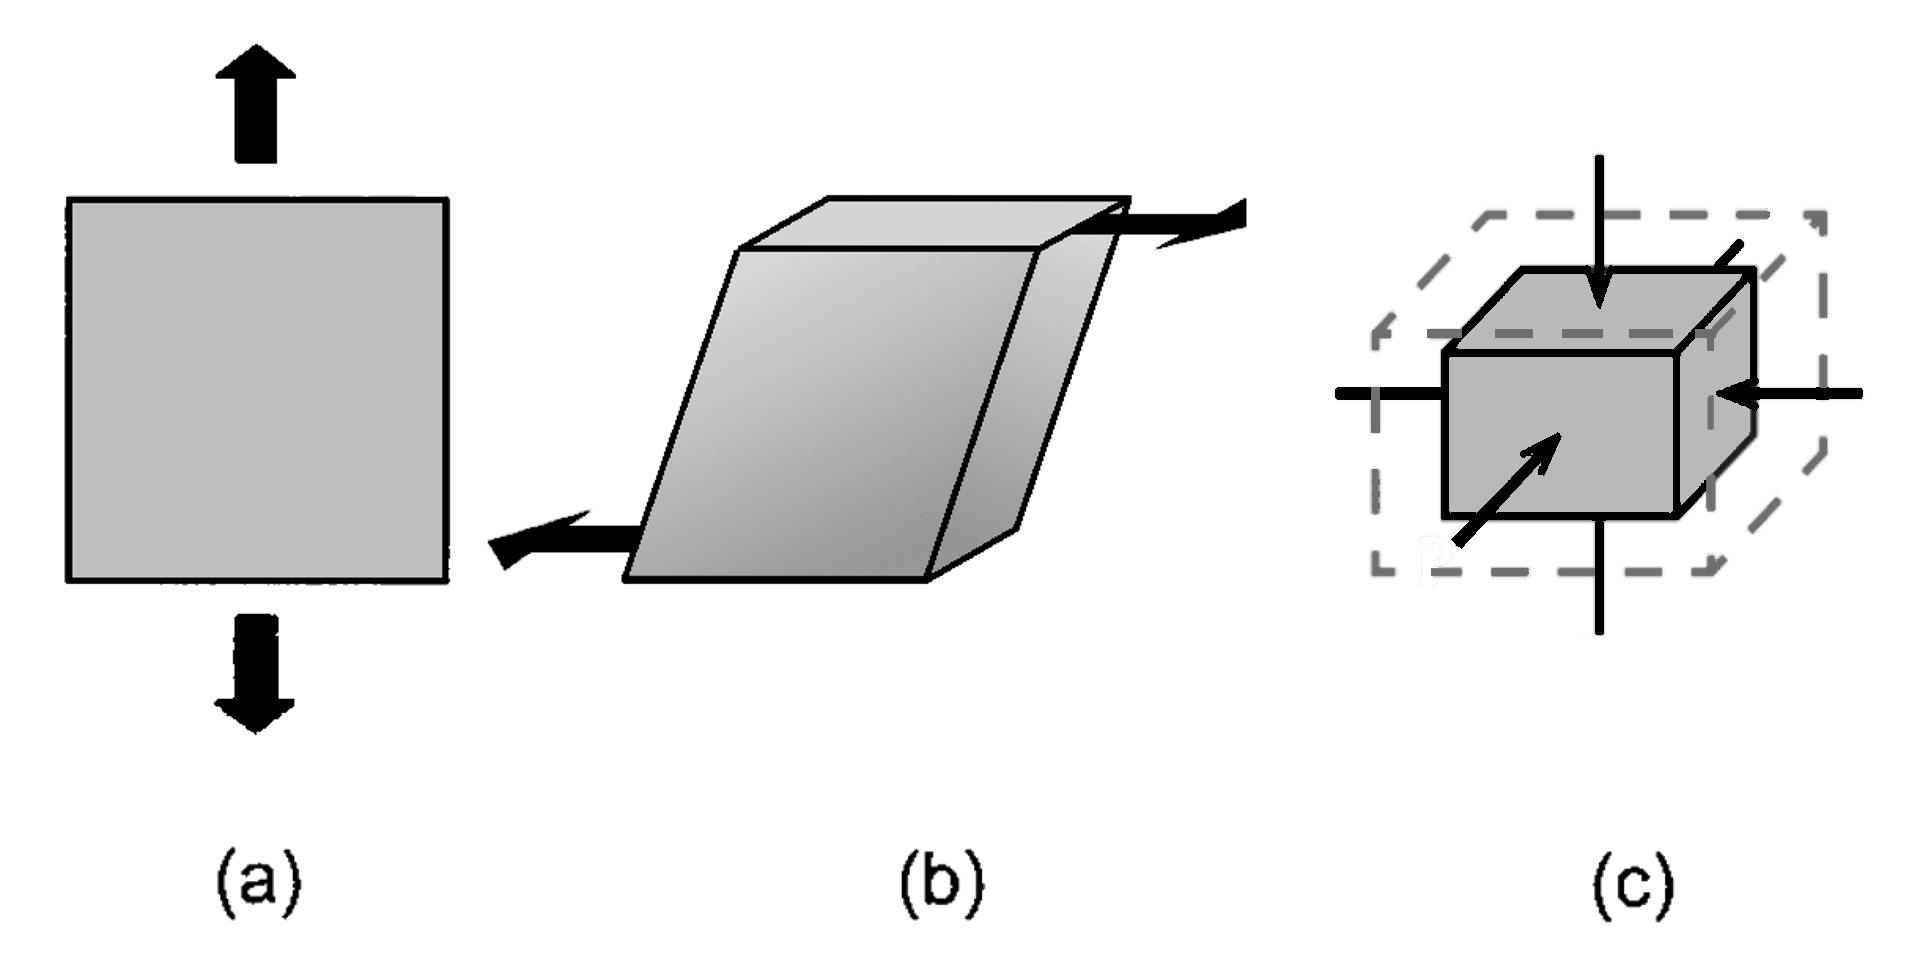
\includegraphics[width=0.7\linewidth]{obrazky/mechanical_tests}
		\caption[Mechanical tests to determine E, K, G moduli]{Mechanical tests to determine (a) E; (b) G; (c) K.}
		\label{fig:mechanicaltests}
	\end{figure}

	%%%%%%%%%%%%%%%%%%%%% SECOND LEVEL %%%%%%%%%%%%%%%%%%%%%%
	\item
	\textit{Second level}, where the constitutive equations must involve two (or more) additional variables. For instance:
	
	\begin{equation}\label{eq:second_level}
		f(\sigma,\varepsilon,\dot{\varepsilon},T, t, c, \Theta)=0,
	\end{equation}
	
	where $\dot{\varepsilon}$ is the strain rate, $T$ means the temperature, $t$ represent time , $c$ is moisture content and $\Theta$ means mechanical dilatation.
	These new variables are necessary for addition viscoelastic behavior into the material model. This behavior is linked to the molecular motions, which are important in the glassy domain (in the Fig. \ref{fig:effectoncrosslinkdensity} between boundaries $\alpha$ and $\beta$). Also they affect the behavior in the glass transition region (around boundary $\alpha$). High influence on the behavior also have thermo-mechanical history from anchor installation and physical aging of the material. 
	For the model are needed also relationships, that describe the effects of $\dot{\varepsilon}$, $\dot{\sigma}$, $T$, $t$, $c$ and $\Theta$ on the previously defined elastic properties. As next will be required equations $J(t)$ (function of compliance, respective creep) and $R(t)$ (function of relaxation), which describe numerical boundary values of elastic properties, which are characterizing unrelaxed a relaxed states.
	
	\begin{figure}
		\centering
		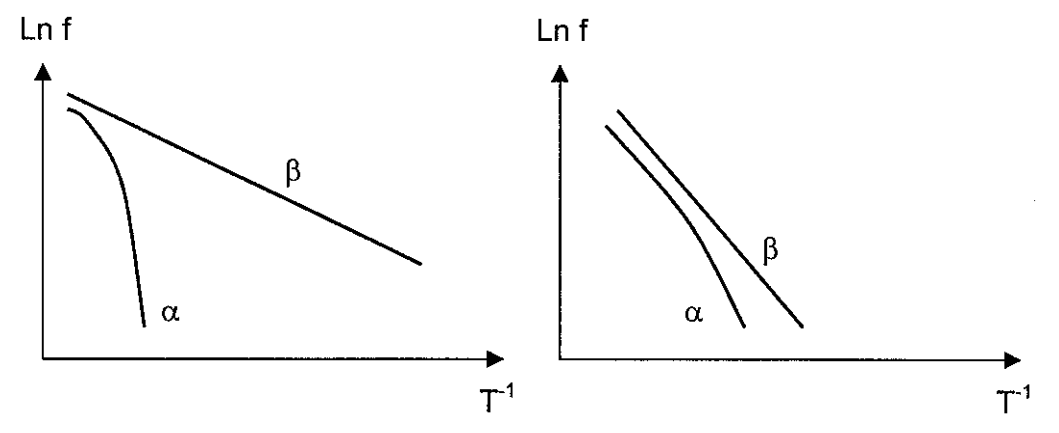
\includegraphics[width=0.8\linewidth]{obrazky/effect_on_cross_link_density}
		\caption[Shape of relaxation maps]{Shape of relaxation maps: dependence of $\ln f$ (frequency) to reciprocal temperature for coordinates of transitions $\alpha$, $\beta$: (a) - polymers having their $\alpha$ and $\beta$ transitions well separated; (b) - polymers with close $\alpha$ and $\beta$ transitions}
		\label{fig:effectoncrosslinkdensity}
	\end{figure}
	
	In the literature we can find three major experimental methods for mechanical characterization in this region, which correspond to particular solutions of the material's state equation: 
	
	\begin{itemize}
		\item Static tests: $\varepsilon = \varepsilon_{0} = constant$ for relaxation, or $\sigma = \sigma_{0} = constant$ for creep. 
		
		\item Monotonous tests with loading rate $\dot{\varepsilon}$, or $\dot{\sigma} = constant$ (for example tensile tests): 
		
		$\dot{\varepsilon} = \dfrac{1}{l}\dfrac{dl}{dt}$
		
		\item dynamic tests: $\varepsilon = \varepsilon_{0} \sin(\omega t)$, or $\sigma = \sigma_{0} \sin(\omega t)$
	\end{itemize}
	
	Polymers are generally assumed to obey the Boltzmann superposition principle in the region of small strains. When there are changes of loading conditions, the effects of these changes are additive when the corresponding responses are considered at equivalent times. For example, if different stresses $\sigma_{0}$, $\sigma_{1}$, $\sigma_{2}$,...$\sigma_{i}$ are applied at different times $0$, $t_{1}$, $t_{2}$,...$t_{i}$, respectively, the final strain is
	
	\begin{equation}\label{eq2:boltzmann_eps}
		\varepsilon(t) = J(t)\sigma_{0} + J(t-t_{1})\sigma_{1}+J(t-t_{2})\sigma_{2}+\cdots+J(t-t_{i})\sigma_{i}
	\end{equation}
	
	where $J(t)$ is the time-dependent creep compliance.
	
	In the same manner, if different strains $\varepsilon_{0}$, $\varepsilon_{1}$, $\varepsilon_{2}$,...$\varepsilon_{i}$ are applied at times $0$, $t_{1}$, $t_{2}$,...$t_{i}$, the final stress is 
	
	\begin{equation}\label{eq2:boltzmann_sig}
	\sigma(t) = E(t)\varepsilon_{0} + E(t-t_{1})\varepsilon_{1}+ E(t-t_{2})\varepsilon_{2}+\cdots+E(t-t_{i})\varepsilon_{i}
	\end{equation}
	
	where $E(t)$ is the time-dependent relaxation modulus. It is generally effective to use dynamic tests to obtain $J(\omega)$ or $E(\omega)$, and then with using mathematical transformations determine $J(t)$ or $E(t)$.
	
	Ordinary, polymers obey a time-temperature superposition principle:
	
	\begin{equation}\label{eq2:shift_factor}
		P_{r}(t,T) = P_{r} \left(\dfrac{t}{a_{T}}, T_{r}\right)
	\end{equation}
	
	where $P_{r}$ is function of $T_{r}$ and $a_{T}$. In Eq. \ref{eq2:shift_factor} $T_{r}$ are a reference temperature and $a_{T}$ is a thermal shift factor, that depend on temperature, humidity and mechanical dilatation. Polymers are interesting in that $a_{T} = f(T, c, \Theta)$ witch take different mathematical forms below and above glass transition temperature $T_{g}$.
	
\end{itemize}


\subsection{Material properties}\label{subsec:mat_proper}
\indent

Material properties, needed for studying model performance of thermosetting polymers, are directly connected to degree of complexity which is being investigated. As you can see in Sec. \ref{sec:poly_complexity}, in the first level basic mechanical properties are needed, e,g. Young modulus $E$ and Poisson's ratio $\nu$. But such low number of material properties makes model limited to relatively sharp intervals of time and temperature, and functioning at low strains.

A higher level of complexity is needed to capture the complicated material behavior. This leads to the more specific material properties, which include yielding and fracture properties, volumetric properties, cohesive properties, glass transition properties, crosslink density, chain mobility, viscoelastic properties,curing degree and aging of the material. Some of them are described below in a more detail.	

\begin{itemize}
	\item 	Yielding properties define boundary between reversible and permanent deformation, but also behavior of the material over this boundary. In normal conditions, the material must be used below the yield boundary, often called elastic limit of material. If the stress goes beyond its yield boundary, the ultimate fracture stress (lost of material integrity) becomes important. Then we need specific theoretical and experimental tools, e.g., fracture mechanics, to study these phenomena.
	
	\item Volumetric properties include free volume, density, packing density and expansion. Free volume is an intrinsic property of the polymer matrix and is created by the gaps left between entangled polymer chains. It can affect absorption and diffusion of the molecules in polymers.
	
	\item Cohesive properties are represented by the cohesive energy as the whole energy of intermolecular interactions, which is easy to determine from calorimetric measurements\footnote{For small molecules}, and cohesive energy density.
	
	\item Glass transition is a catastrophic softening of the material, when temperature is higher then the glass transition temperature $T_g$. Also has influence to the curing process due to its exothermal behavior. 
	
	\item Viscoelastic properties include creep and relaxation properties, which describe connections between the stresses and strains with respect to time. Creep means increasing of the strains in time with constant stress and relaxation means reduction of the stresses under constant strains. 
	
	\item Curing degree defines change of the material from the liquid to the glassy state. Note that bonded anchors have an uncertain curing degree of the mortar when they are loaded.
	
\end{itemize}

